\documentclass[a4paper,11pt]{article}

% ---------------------------
%         Packages
% ---------------------------
\usepackage{tikz}
\usepackage{fullpage}
\usepackage{amsmath,amsthm,amsfonts,amssymb,amscd}
\usepackage{mathtools}
\usepackage{colortbl}
\usepackage{xcolor}
\usepackage{graphicx}
\usepackage{titlesec}
\usepackage{multirow}
\usepackage{booktabs}
\usepackage{listings}
\usepackage{float}
\usepackage{hyperref}
\usepackage{geometry}
\usepackage{array}
\usepackage{tabularx}
\usepackage{pifont}

\usepackage{xepersian}

% ---------------------------
%      Dark Theme Setup
% ---------------------------
\definecolor{CustomBackground}{HTML}{1C1C1C}
\definecolor{AccentBlue}{HTML}{4FA3D1}
\definecolor{AccentGreen}{HTML}{5DBB8A}
\definecolor{LightGray}{HTML}{CCCCCC}
\definecolor{MidGray}{HTML}{888888}
\definecolor{CodeBg}{HTML}{111111}

\pagecolor{CustomBackground}
\color{white}
\arrayrulecolor{white}

\hypersetup{
    colorlinks=true,
    linkcolor=AccentBlue,
    urlcolor=AccentBlue,
    citecolor=AccentGreen
}

% ---------------------------
%        Font Setup
% ---------------------------
\settextfont{Vazir.ttf}[
    BoldFont = Vazir-Bold.ttf,
    Path = fonts/
]

% ---------------------------
%       Page Geometry
% ---------------------------
\geometry{
    a4paper,
    top=2.5cm,
    bottom=2.5cm,
    left=2.5cm,
    right=2.5cm
}

% ---------------------------
%     Section Formatting
% ---------------------------
\renewcommand{\baselinestretch}{1.3}
\renewcommand{\thesection}{\arabic{section}}

\titleformat{\section}
    {\Large\bfseries\color{AccentBlue}}
    {\thesection.}{0.5em}{}[\titlerule]

\titleformat{\subsection}
    {\large\bfseries\color{AccentGreen}}
    {\thesubsection.}{0.5em}{}

\titleformat{\subsubsection}
    {\normalsize\bfseries\color{LightGray}}
    {\thesubsubsection.}{0.5em}{}

% ---------------------------
%       Code Listings
% ---------------------------
\lstset{
    basicstyle=\ttfamily\small\color{white},
    breaklines=true,
    frame=single,
    rulecolor=\color{MidGray},
    backgroundcolor=\color{CodeBg},
    keywordstyle=\color{AccentBlue}\bfseries,
    commentstyle=\color{AccentGreen},
    stringstyle=\color{yellow},
    numberstyle=\tiny\color{MidGray},
    numbers=left,
    stepnumber=1,
    columns=fullflexible,
    keepspaces=true,
    showstringspaces=false
}

% ---------------------------
%       Custom Commands
% ---------------------------
\newcommand{\coursename}{مبانی هوش محاسباتی}
\newcommand{\projecttitle}{\lr{Persian Sentiment Analysis with Ensemble Learning}}
\newcommand{\profname}{دکتر فضل ارثی}
\newcommand{\deptname}{گروه مهندسی کامپیوتر}
\newcommand{\univname}{دانشگاه فردوسی مشهد}
\newcommand{\semestername}{نیمسال دوم \lr{1404}–\lr{1405}}

% Student info
\newcommand{\studentOneID}{\lr{4022262035}}
\newcommand{\studentOneName}{امیرحسین ابوالفضلی}
\newcommand{\studentOneEmail}{\lr{abolfazli2035@gmail.com}}

\newcommand{\studentTwoID}{\lr{4021262131}}
\newcommand{\studentTwoName}{آرمان بیجاری}
\newcommand{\studentTwoEmail}{\lr{armanbijari5@gmail.com}}

% ---------------------------
%           Document
% ---------------------------
\begin{document}

% =================================
%           Title Page
% =================================
\begin{titlepage}
    \begin{center}

        
\includegraphics[scale=1.1]{assets/fum-logo.png}\\[0.8cm]

        {\Large\bfseries \univname}\\[0.2cm]
        {\large \deptname}\\[0.6cm]

        \textcolor{AccentBlue}{\rule{0.8\linewidth}{0.6pt}}\\[0.6cm]

        {\large گزارش پروژه درس}\\[0.3cm]
        {\Huge\bfseries \coursename}\\[0.5cm]

        \textcolor{AccentBlue}{\rule{0.8\linewidth}{0.6pt}}\\[0.8cm]

        {\LARGE\bfseries \projecttitle}\\[0.4cm]
        {\large\color{LightGray} تحلیل احساسات نظرات فارسی با یادگیری ترکیبی}\\[2cm]

        \begin{tabular}{r|l}
            \textbf{نام و نام خانوادگی} & \textbf{شماره دانشجویی} \\[4pt]
            \hline\\[-6pt]
            \studentOneName & \studentOneID \\[4pt]
            \studentTwoName & \studentTwoID \\
        \end{tabular}

        \vspace{1.5cm}

        {\large استاد: \textbf{\profname}}\\[0.5cm]
        {\color{MidGray} \semestername}

    \end{center}
\end{titlepage}

% =================================
%        Table of Contents
% =================================
\tableofcontents
\newpage

% =================================
%            Sections
% =================================
\section{معرفی داده‌ها}

داده‌ای که توی این پروژه باهاش کار کردیم \lr{Snapfood Persian Sentiment Analysis} هستش که از \lr{Kaggle}\footnote{\lr{Kaggle}: پلتفرم آنلاین برای مسابقات یادگیری ماشین و به اشتراک‌گذاری دیتاست.} برداشتیم. داده \lr{70,000} تا نظر کاربرای \lr{Snapfood} داره که بعد از سفارش غذا نوشتن. هر نظر یه برچسب داره: \lr{HAPPY} (مثبت) یا \lr{SAD} (منفی). بعد از فیلتر اولیه \lr{69,480} ردیف مونده (\lr{HAPPY}: \lr{34,916} / \lr{SAD}: \lr{34,564}) و بعد از پاکسازی \lr{69,479} ردیف (\lr{1} نظر خالی حذف شد). از نظر تعداد کلاس متوازنه.

یه چیزی که داده رو جالب و در عین حال چالش‌برانگیز می‌کنه اینه که نظرات کاملاً واقعی و عامیانه‌ان. غلط نگارشی، کشیدن حروف، \lr{emoji}، قاطی فارسی-انگلیسی، همه هست. اینا نویز حساب میشن ولی بخشی‌شون خودش سیگنال احساسه.

\begin{figure}[H]
    \centering
    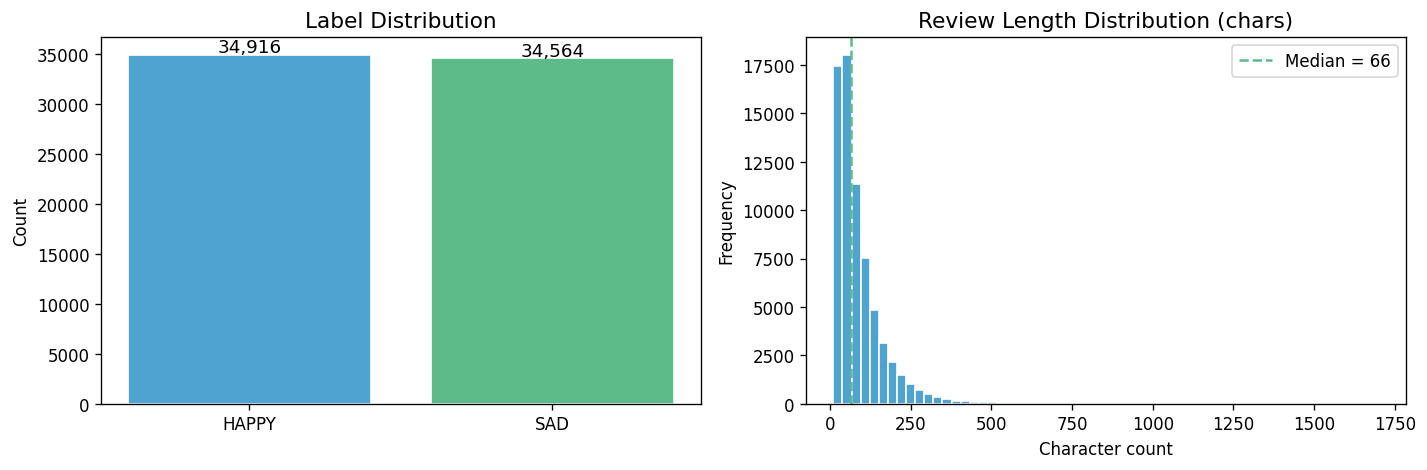
\includegraphics[width=0.7\textwidth]{../outputs/figures/eda_distribution.png}
    \caption{توزیع برچسب‌های مثبت و منفی در داده}
    \label{fig:eda_dist}
\end{figure}

پس داده خوبیه، ولی چون عامیانه و غیررسمیه، پیش‌پردازش درست خیلی مهمه.

یه چیز دیگه که توی ارزیابی مدل خیلی اثر میذاره اینه که برچسب‌ها همیشه تمیز نیستن. حدود \lr{22\%} نظرها «ولی» یا «اما» دارن؛ حدود \lr{6\%} همزمان کلمات مثبت و منفی دارن. برای انسان قابل فهمه، ولی برای مدلی که فقط یه برچسب \lr{HAPPY}/\lr{SAD} می‌بینه گیج‌کننده‌ست. پس سقف دقت فقط با مدل بهتر بالا نمیره، بخشی‌ش سقف ذاتی برچسب‌گذاریه.


\section{فاز اول: پیش‌پردازش متن}

\subsection{چرا فارسی سخت‌تره؟}

یه مشکل خاص فارسی اینه که بعضی حروف با عربی یونیکد مشترک ندارن ولی عین هم به نظر میان. «ی» فارسی \lr{U+06CC} و «ي» عربی \lr{U+064A}. از دید مدل دو کلمه جدا میشن مگر اینکه اول نرمال‌سازی کنیم.

\subsection{مراحل پیش‌پردازش}

کد توی \lr{\texttt{src/preprocessing.py}} هست. برخلاف یه pipeline عمومی، اینجا عمداً سیگنال احساس رو نگه می‌داریم:
اول \lr{URL} حذف میشه (قبل از \lr{Hazm}\footnote{\lr{Hazm}: کتابخونه پایتون برای پردازش زبان طبیعی فارسی.} چون نرمالایزر \lr{://} رو می‌بلعه). بعد \lr{emoji}های احساسی به \lr{EMO\_POS}/\lr{EMO\_NEG} نگاشت میشن، نه اینکه کورکورانه حذف بشن. نرمال‌سازی فارسی، حذف اعداد و علائم، جمع‌کردن حروف تکراری (خوووب $\rightarrow$ خوب)، توکن‌سازی، و مهم‌تر از همه \textbf{برچسب‌گذاری نفی}: بعد نفی‌کننده‌ها مثل «نه» به کلمات بعدی پیشوند \lr{NEG\_} می‌خوره (ایده \lr{Pang \& Lee}). حذف \lr{stopword} پیش‌فرض \textbf{خاموش}ه چون لیست \lr{Hazm} نفی‌کننده و شدت‌دهنده داره. آخر سر \lr{lemmatization} با \lr{Hazm.Lemmatizer()}؛ توکن‌های \lr{EMO\_}/\lr{NEG\_} دست نمی‌خورن.

\subsection{نمونه‌هایی از قبل و بعد}

\begin{table}[H]
\centering
\small
\begin{tabularx}{\textwidth}{X X}
\toprule
\textbf{متن اصلی} & \textbf{بعد از پیش‌پردازش} \\
\midrule
سلام خیلی خوووووب بود! غذا عالیییی بود & سلام خیلی خوب بود غذا عالی بود \\
\addlinespace
بدترین تجربه زندگیم بود. اصلا توصیه نمیکنم & بدترین تجربه زندگیم بود اصلا توصیه کرد به هیچ کس \\
\addlinespace
غذا وقتی رسید سرد بوووووود. افتضاح & غذا وقتی رسید سرد بوود افتضاح \\
\bottomrule
\end{tabularx}
\caption{نمونه‌های واقعی از نوت‌بوک فاز اول}
\label{tab:preprocessing_examples}
\end{table}

\begin{figure}[H]
    \centering
    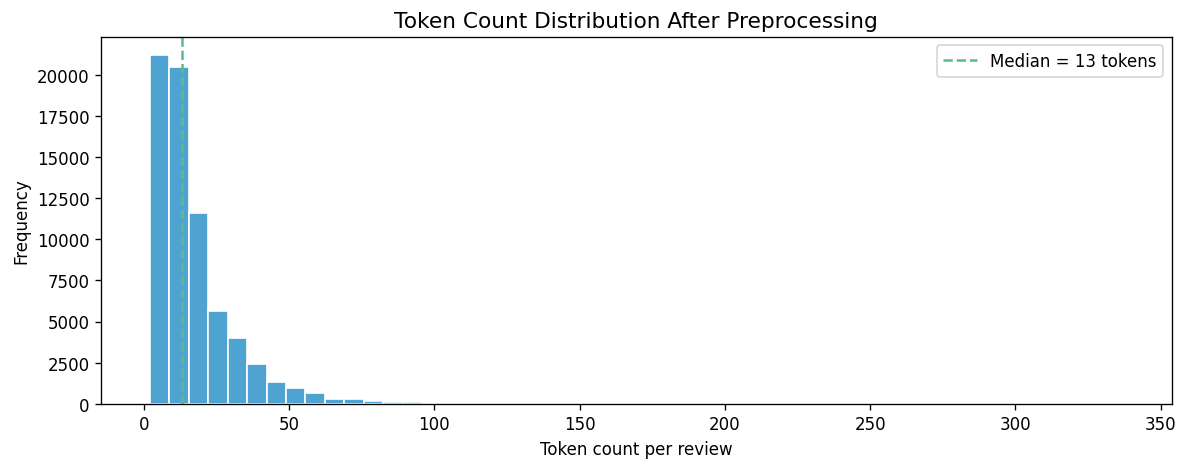
\includegraphics[width=0.65\textwidth]{../outputs/figures/token_distribution.png}
    \caption{توزیع تعداد توکن (میانگین \lr{17}، میانه \lr{13})}
    \label{fig:token_dist}
\end{figure}

\subsection{تقسیم داده}

با \lr{stratified split}\footnote{\lr{stratified split}: نسبت کلاس‌ها توی train و test یکی بمونه.} و \lr{random\_state=42}: آموزش \lr{55,583} (\lr{HAPPY} \lr{27,933} / \lr{SAD} \lr{27,650})، آزمون \lr{13,896} (\lr{HAPPY} \lr{6,983} / \lr{SAD} \lr{6,913}). میانگین طول متن \lr{89.7} کاراکتر (میانه \lr{66}).


\section{فاز دوم: \lr{Vectorization}}

سه روش اجباری پروژه رو پیاده کردیم، به علاوه دو نمایش bonus که توی فازهای بعدی مقایسه شدن.

\subsection{\lr{CountVectorizer} و \lr{TF-IDF}}

هر دو sparse با \lr{max\_features=50,000}، \lr{ngram\_range=(1,2)}، \lr{min\_df=2}. \lr{TF-IDF} با \lr{sublinear\_tf=True}. هر دو ماتریس \lr{50,000} بعدی با پراکندگی \lr{99.9466\%} ساختن.

\subsection{\lr{Word2Vec}}

\lr{Skip-gram}، \lr{vector\_size=100}، آموزش از صفر روی کورپوس. میانگین بردار کلمات برای هر سند. \lr{OOV} روی train حدود \lr{53.9\%} — برای نظرات کوتاه و عامیانه طبیعیه.

\subsection{نمایش‌های bonus}

\lr{Word2Vec-IDF}: میانگین وزن‌دار با \lr{IDF} (ایده شبیه \lr{SIF}). \lr{Hybrid word+char TF-IDF}: اتحاد \lr{word} و \lr{char\_wb} n-gram؛ \lr{101,119} بعد با پراکندگی \lr{99.7875\%}. برای املای غلط و کشیدگی فارسی خیلی کمک می‌کنه.

\begin{table}[H]
\centering
\small
\begin{tabular}{lccc}
\toprule
\textbf{نمایش} & \textbf{بعد} & \textbf{نوع} & \textbf{پراکندگی} \\
\midrule
\lr{CountVectorizer} & \lr{50,000} & sparse & \lr{99.9466\%} \\
\lr{TF-IDF} & \lr{50,000} & sparse & \lr{99.9466\%} \\
\lr{Word2Vec (mean)} & \lr{100} & dense & --- \\
\lr{Word2Vec-IDF} & \lr{100} & dense & --- \\
\lr{Hybrid} & \lr{101,119} & sparse & \lr{99.7875\%} \\
\bottomrule
\end{tabular}
\caption{خلاصه نمایش‌های عددی}
\label{tab:vec_summary}
\end{table}

\begin{figure}[H]
    \centering
    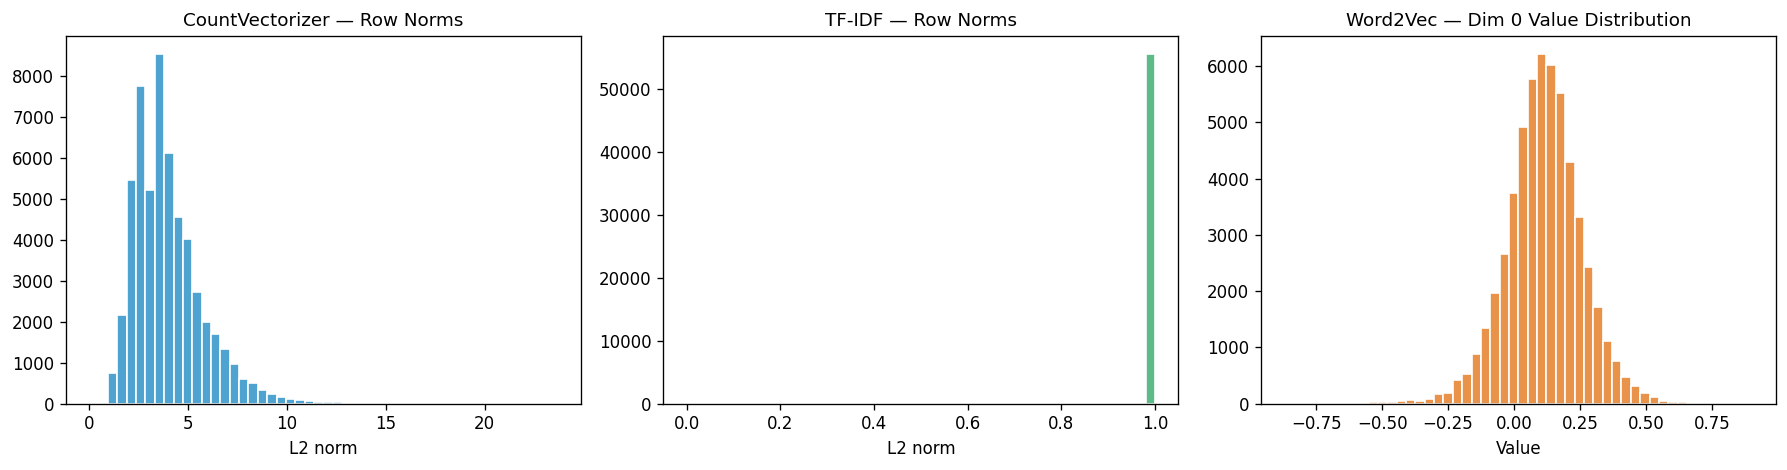
\includegraphics[width=0.7\textwidth]{../outputs/figures/vectorizer_norms.png}
    \caption{توزیع نُرم بردارها}
    \label{fig:vec_norms}
\end{figure}


\section{فاز سوم: آموزش و ارزیابی مدل‌های پایه}

\subsection{مدل‌ها و تنظیمات}

\lr{9} مدل کلاسیک روی پنج \lr{vectorizer} (سه اجباری + دو bonus): \lr{ComplementNB}، \lr{GaussianNB}، \lr{SVM (Linear)} داخل \lr{CalibratedClassifierCV}، \lr{LogisticRegression}، \lr{DecisionTree}، \lr{RandomForest}، \lr{KNN}، \lr{AdaBoost}، \lr{HistGradientBoosting}. \lr{ComplementNB} فقط روی sparse غیرمنفی؛ \lr{GaussianNB} روی \lr{Word2Vec}؛ \lr{HistGradBoost} روی dense. جمعاً \lr{32} آزمایش در sweep اولیه، بعد \lr{GridSearchCV} برای سه مدل خطی/NB برتر.

\begin{table}[H]
\centering
\small
\begin{tabularx}{\textwidth}{l X}
\toprule
\textbf{مدل} & \textbf{تنظیمات sweep} \\
\midrule
\lr{ComplementNB / GaussianNB} & \lr{alpha=0.1} \\
\lr{SVM (Linear)} & \lr{C=1.0, max\_iter=4000} در \lr{CalibratedClassifierCV} \\
\lr{LogisticRegression} & \lr{C=1.0, solver=lbfgs} \\
\lr{Random Forest} & \lr{n\_estimators=200} \\
\lr{HistGradientBoosting} & \lr{max\_iter=400} (فقط dense) \\
\lr{KNN} & \lr{n\_neighbors=7, metric=cosine} \\
\bottomrule
\end{tabularx}
\caption{مدل‌های پایه}
\label{tab:model_configs}
\end{table}

\subsection{نتایج کامل}

جدول زیر همه \lr{32} ترکیب (شامل سه مدل tune‌شده در انتها) رو بر اساس \lr{F1} مرتب کرده:

\begin{table}[H]
\centering
\scriptsize
\begin{tabular}{llcccc}
\toprule
\textbf{مدل} & \textbf{\lr{Vectorizer}} & \textbf{دقت} & \textbf{صحت} & \textbf{فراخوانی} & \textbf{\lr{F1}} \\
\midrule
\lr{SVM\_(Linear)\_(tuned)} & \lr{Hybrid} & \lr{0.8578} & \lr{0.8620} & \lr{0.8578} & \lr{0.8574} \\
\lr{LogisticReg\_(tuned)} & \lr{Hybrid} & \lr{0.8569} & \lr{0.8602} & \lr{0.8569} & \lr{0.8566} \\
\lr{LogisticReg} & \lr{Hybrid} & \lr{0.8565} & \lr{0.8589} & \lr{0.8565} & \lr{0.8563} \\
\lr{LogisticReg} & \lr{TF-IDF} & \lr{0.8554} & \lr{0.8590} & \lr{0.8554} & \lr{0.8551} \\
\lr{ComplementNB\_(tuned)} & \lr{CountVectorizer} & \lr{0.8505} & \lr{0.8545} & \lr{0.8505} & \lr{0.8501} \\
\lr{ComplementNB} & \lr{CountVectorizer} & \lr{0.8491} & \lr{0.8534} & \lr{0.8491} & \lr{0.8487} \\
\lr{RandomForest} & \lr{CountVectorizer} & \lr{0.8487} & \lr{0.8530} & \lr{0.8487} & \lr{0.8483} \\
\lr{SVM\_(Linear)} & \lr{Hybrid} & \lr{0.8464} & \lr{0.8480} & \lr{0.8464} & \lr{0.8463} \\
\lr{ComplementNB} & \lr{TF-IDF} & \lr{0.8462} & \lr{0.8525} & \lr{0.8462} & \lr{0.8456} \\
\lr{SVM\_(Linear)} & \lr{TF-IDF} & \lr{0.8449} & \lr{0.8467} & \lr{0.8449} & \lr{0.8448} \\
\lr{RandomForest} & \lr{TF-IDF} & \lr{0.8446} & \lr{0.8503} & \lr{0.8446} & \lr{0.8440} \\
\lr{LogisticReg} & \lr{CountVectorizer} & \lr{0.8429} & \lr{0.8436} & \lr{0.8429} & \lr{0.8428} \\
\lr{ComplementNB} & \lr{Hybrid} & \lr{0.8416} & \lr{0.8489} & \lr{0.8416} & \lr{0.8408} \\
\lr{LogisticReg} & \lr{Word2Vec} & \lr{0.8397} & \lr{0.8427} & \lr{0.8397} & \lr{0.8394} \\
\lr{SVM\_(Linear)} & \lr{Word2Vec} & \lr{0.8392} & \lr{0.8421} & \lr{0.8392} & \lr{0.8389} \\
\lr{HistGradBoost} & \lr{Word2Vec} & \lr{0.8381} & \lr{0.8417} & \lr{0.8381} & \lr{0.8377} \\
\lr{RandomForest} & \lr{Word2Vec} & \lr{0.8344} & \lr{0.8419} & \lr{0.8344} & \lr{0.8336} \\
\lr{SVM\_(Linear)} & \lr{Word2Vec-IDF} & \lr{0.8315} & \lr{0.8344} & \lr{0.8315} & \lr{0.8312} \\
\lr{LogisticReg} & \lr{Word2Vec-IDF} & \lr{0.8315} & \lr{0.8345} & \lr{0.8315} & \lr{0.8311} \\
\lr{HistGradBoost} & \lr{Word2Vec-IDF} & \lr{0.8285} & \lr{0.8318} & \lr{0.8285} & \lr{0.8281} \\
\lr{SVM\_(Linear)} & \lr{CountVectorizer} & \lr{0.8267} & \lr{0.8272} & \lr{0.8267} & \lr{0.8267} \\
\lr{AdaBoost} & \lr{Word2Vec} & \lr{0.8217} & \lr{0.8244} & \lr{0.8217} & \lr{0.8214} \\
\lr{KNN} & \lr{Word2Vec} & \lr{0.8185} & \lr{0.8227} & \lr{0.8185} & \lr{0.8180} \\
\lr{AdaBoost} & \lr{CountVectorizer} & \lr{0.8051} & \lr{0.8200} & \lr{0.8051} & \lr{0.8030} \\
\lr{GaussianNB} & \lr{Word2Vec} & \lr{0.8020} & \lr{0.8251} & \lr{0.8020} & \lr{0.7985} \\
\lr{KNN} & \lr{TF-IDF} & \lr{0.7979} & \lr{0.7999} & \lr{0.7979} & \lr{0.7976} \\
\lr{DecisionTree} & \lr{TF-IDF} & \lr{0.7988} & \lr{0.8148} & \lr{0.7988} & \lr{0.7963} \\
\lr{DecisionTree} & \lr{CountVectorizer} & \lr{0.7962} & \lr{0.8074} & \lr{0.7962} & \lr{0.7945} \\
\lr{AdaBoost} & \lr{TF-IDF} & \lr{0.7957} & \lr{0.8167} & \lr{0.7957} & \lr{0.7924} \\
\lr{GaussianNB} & \lr{Word2Vec-IDF} & \lr{0.7855} & \lr{0.8088} & \lr{0.7855} & \lr{0.7816} \\
\lr{KNN} & \lr{CountVectorizer} & \lr{0.7686} & \lr{0.7752} & \lr{0.7686} & \lr{0.7671} \\
\lr{DecisionTree} & \lr{Word2Vec} & \lr{0.7475} & \lr{0.7476} & \lr{0.7475} & \lr{0.7475} \\
\bottomrule
\end{tabular}
\caption{نتایج کامل \lr{32} آزمایش}
\label{tab:full_results}
\end{table}

\begin{figure}[H]
    \centering
    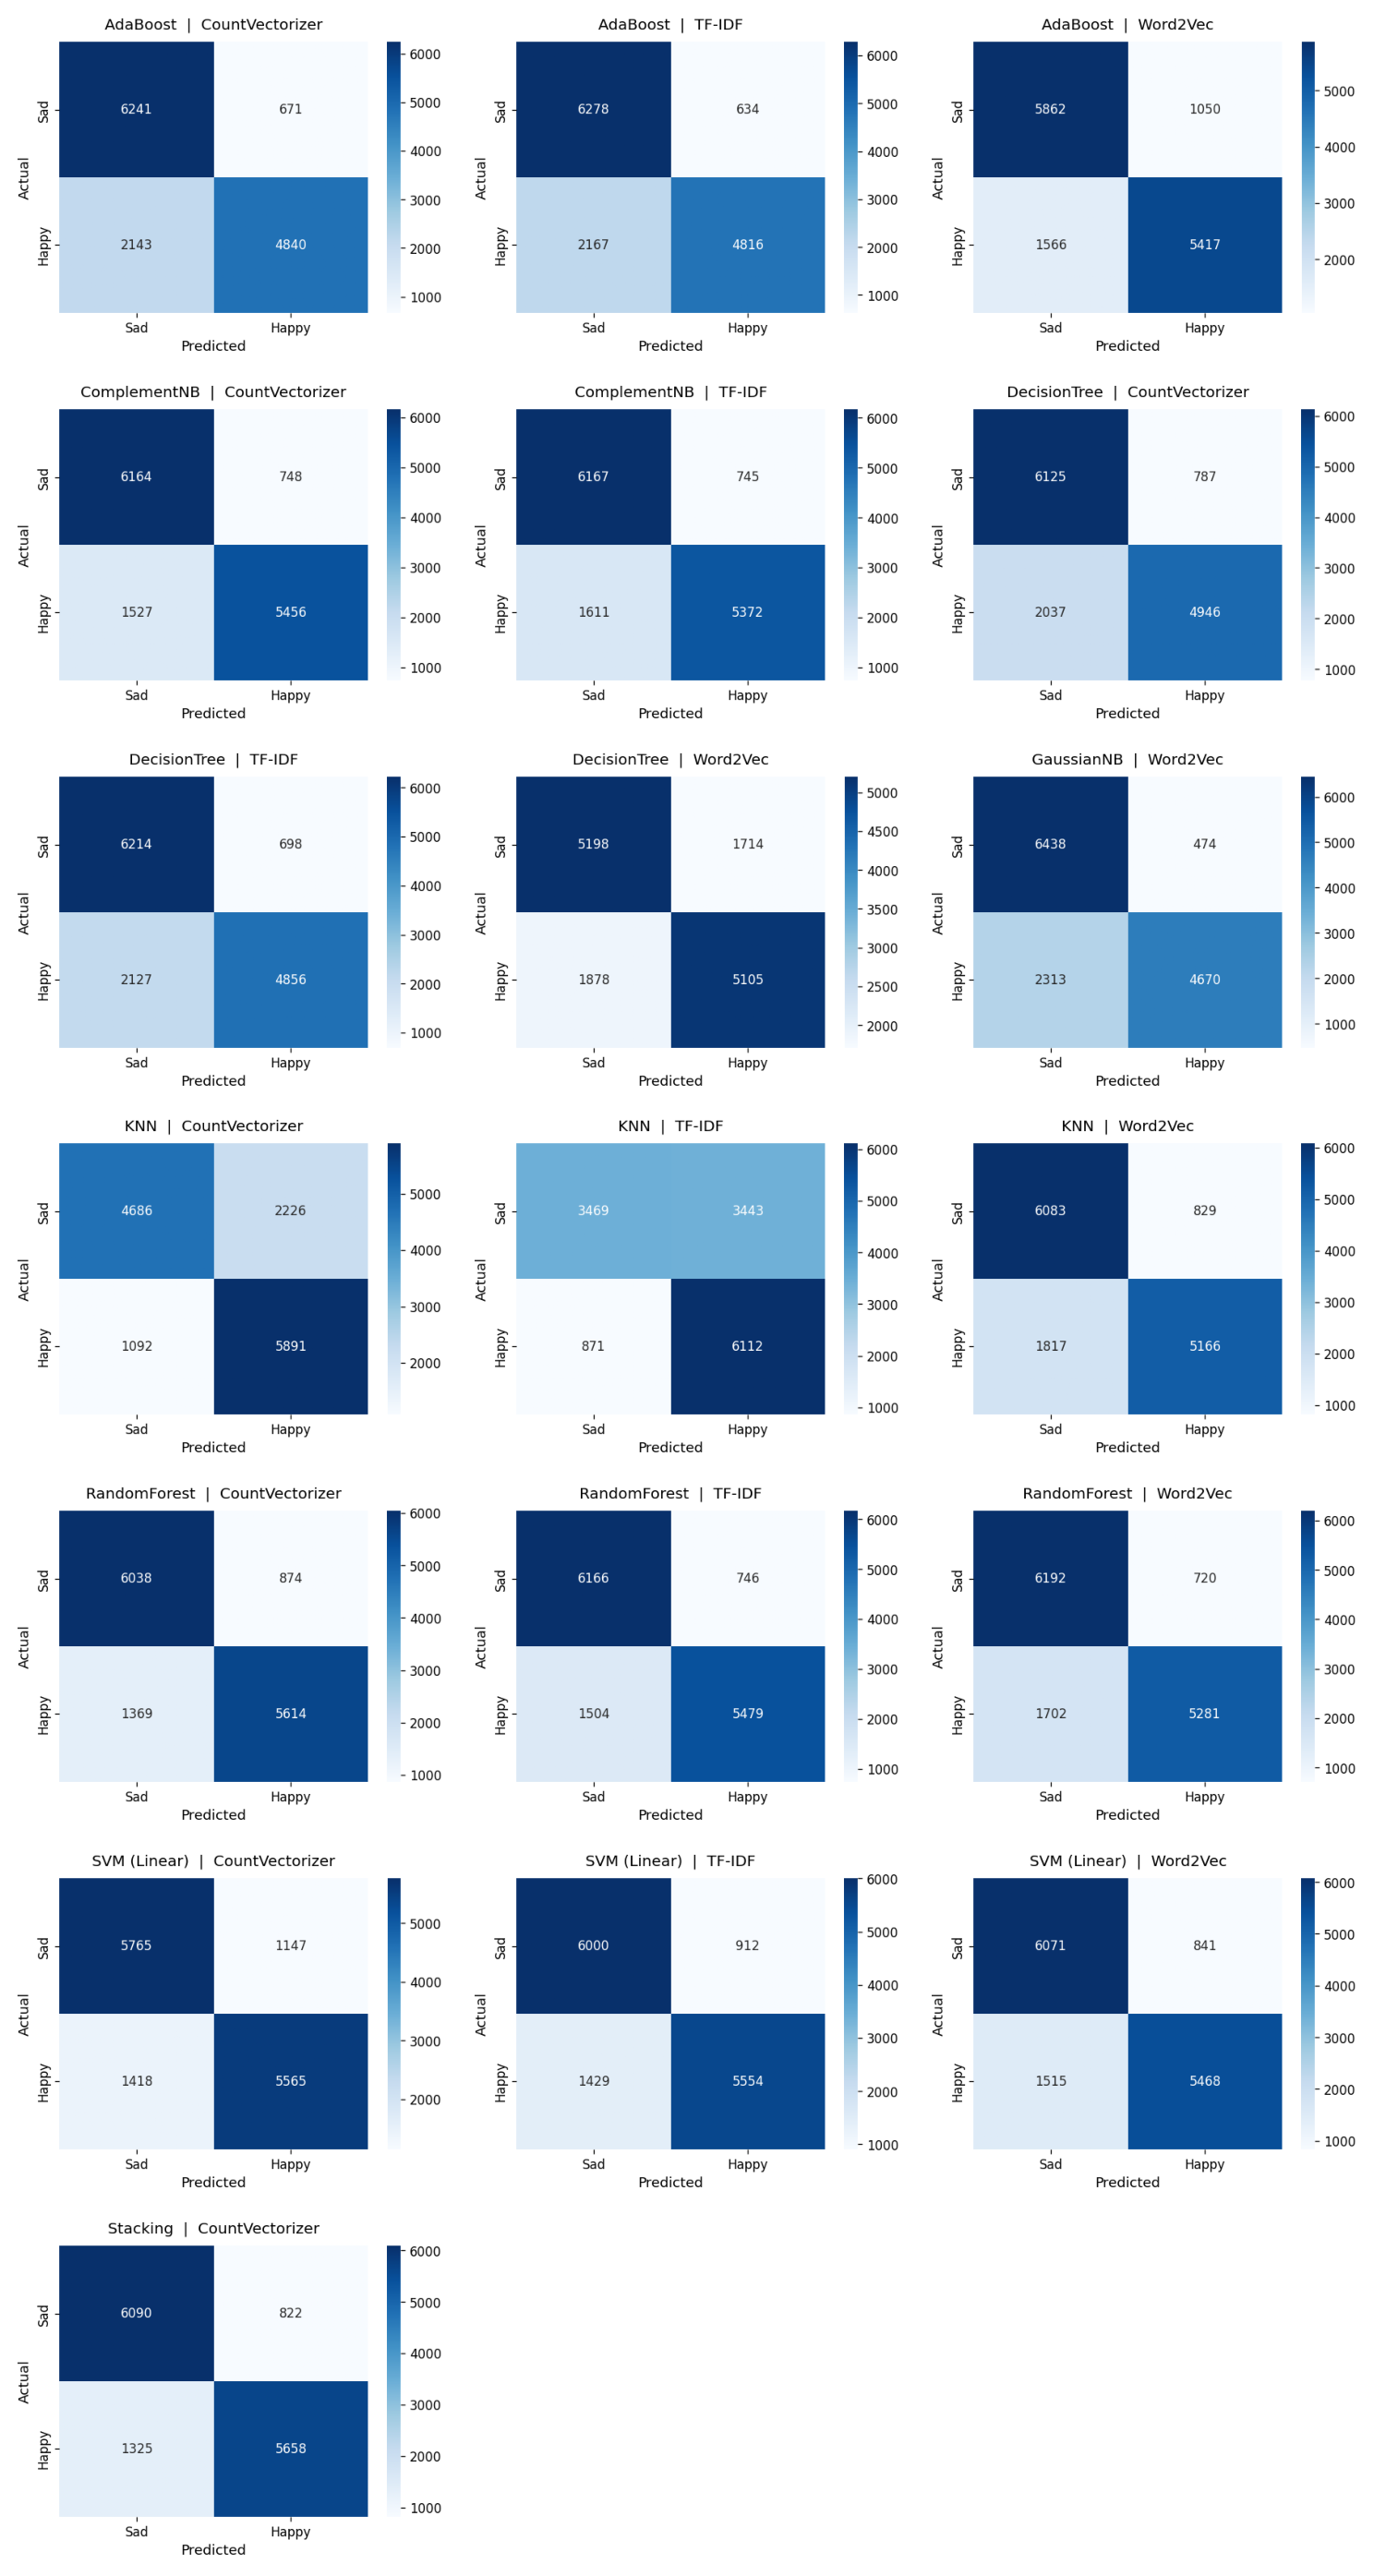
\includegraphics[width=0.5\textwidth]{../outputs/figures/all_confusion_matrices.png}
    \caption{ماتریس درهم‌ریختگی همه مدل‌ها}
    \label{fig:all_cms}
\end{figure}

\begin{figure}[H]
    \centering
    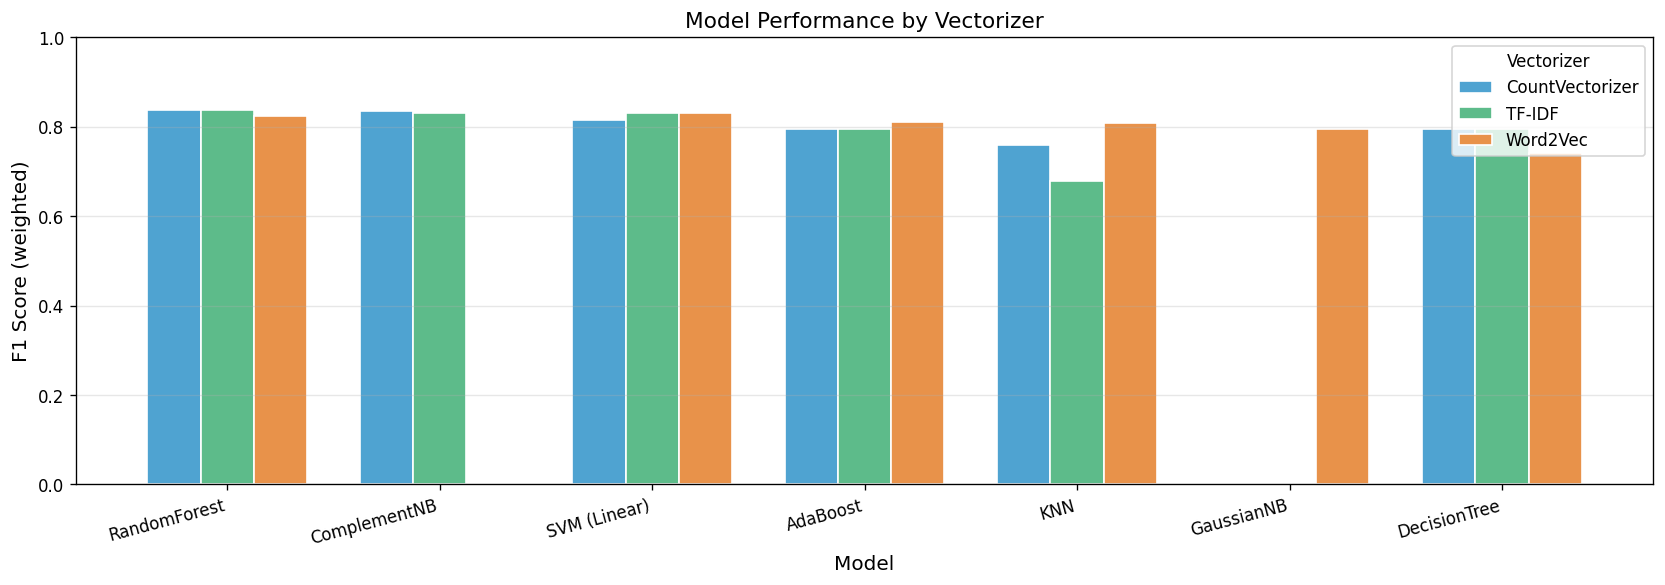
\includegraphics[width=\textwidth]{../outputs/figures/phase3_f1_comparison.png}
    \caption{مقایسه \lr{F1} روی پنج \lr{vectorizer}}
    \label{fig:f1_comparison}
\end{figure}

\subsection{تحلیل نتایج}

بهترین ترکیب بعد از \lr{GridSearchCV}: \lr{SVM (Linear) (tuned)} روی \lr{Hybrid} با \lr{F1=0.8574} و دقت \lr{0.8578}. \lr{LogisticRegression} روی \lr{Hybrid} و \lr{TF-IDF} هم نزدیک (\lr{0.8563} و \lr{0.8551}). \lr{Random Forest} دیگه برنده نیست؛ روی sparseهای پُربُعد، مدل‌های خطی با \lr{C} درست قوی‌ترن.

بدترین‌ها همچنان \lr{DecisionTree} روی \lr{Word2Vec} (\lr{F1=0.7475}) و \lr{KNN} روی sparse (\lr{0.7671} روی \lr{CountVectorizer}). \lr{KNN} توی فضای \lr{50k}-بعدی sparse گم میشه.

\subsection{تنظیم ابرپارامتر و ablation پیش‌پردازش}

\lr{GridSearchCV} با \lr{5}-fold: \lr{ComplementNB} \lr{alpha=1.0} روی \lr{CountVectorizer} (\lr{F1=0.8501})؛ \lr{SVM} \lr{C=0.05} روی \lr{Hybrid} (\lr{0.8574})؛ \lr{LogisticReg} \lr{C=0.5} (\lr{0.8566}).

روی زیرنمونه \lr{15k/5k}، حذف \lr{lemmatization} (\lr{F1=0.8572}) از pipeline فعلی (\lr{0.8512}) جلو بود، ولی pipeline فعلی رو نگه داشتیم چون ablation کوچک بود و negation/emoji-mapping عمداً برای احساس طراحی شده.

\subsection{نمونه پیش‌بینی‌های اشتباه (بهترین مدل sweep)}

\begin{table}[H]
\centering
\small
\begin{tabularx}{\textwidth}{X c c}
\toprule
\textbf{متن} & \textbf{برچسب} & \textbf{پیش‌بینی} \\
\midrule
کیفیت خوب بود ولی نسبت به قیمت حجم غذا خوب بود & \lr{SAD} & \lr{HAPPY} \\
هسته زردآلو خیلی بد بود ولی برگه هلو خوب بود & \lr{SAD} & \lr{HAPPY} \\
سالاد سزار کاهو موند رنگ عوض شد سیب‌زمینی ساده خوب بود & \lr{HAPPY} & \lr{SAD} \\
\bottomrule
\end{tabularx}
\caption{خطاهای \lr{LogisticReg + Hybrid} — الگوی «ولی»}
\label{tab:prediction_examples}
\end{table}

پس برنده sweep اولیه \lr{LogisticReg + Hybrid} بود (\lr{0.8563})؛ بعد از tune، \lr{SVM + Hybrid} به \lr{0.8574} رسید.


\section{فاز چهارم: انتخاب بهترین \lr{Vectorizer}}

\subsection{میانگین و اوج عملکرد}

\begin{table}[H]
\centering
\begin{tabular}{lcccc}
\toprule
\textbf{\lr{Vectorizer}} & \textbf{دقت} & \textbf{صحت} & \textbf{فراخوانی} & \textbf{\lr{F1}} \\
\midrule
\lr{Hybrid} & \lr{0.8518} & \lr{0.8556} & \lr{0.8518} & \lr{0.8515} \\
\lr{TF-IDF} & \lr{0.8262} & \lr{0.8343} & \lr{0.8262} & \lr{0.8251} \\
\lr{CountVectorizer} & \lr{0.8235} & \lr{0.8293} & \lr{0.8235} & \lr{0.8226} \\
\lr{Word2Vec-IDF} & \lr{0.8193} & \lr{0.8274} & \lr{0.8193} & \lr{0.8180} \\
\lr{Word2Vec} & \lr{0.8176} & \lr{0.8235} & \lr{0.8176} & \lr{0.8169} \\
\bottomrule
\end{tabular}
\caption{میانگین \lr{F1} روی همه مدل‌های هر \lr{vectorizer}}
\label{tab:vec_avg}
\end{table}

\begin{table}[H]
\centering
\begin{tabular}{lc}
\toprule
\textbf{\lr{Vectorizer}} & \textbf{اوج \lr{F1}} \\
\midrule
\lr{Hybrid} & \lr{0.8574} \\
\lr{TF-IDF} & \lr{0.8551} \\
\lr{CountVectorizer} & \lr{0.8501} \\
\lr{Word2Vec} & \lr{0.8394} \\
\lr{Word2Vec-IDF} & \lr{0.8312} \\
\bottomrule
\end{tabular}
\caption{بالاترین \lr{F1} هر نمایش (بعد از tune)}
\label{tab:peak_f1}
\end{table}

\begin{figure}[H]
    \centering
    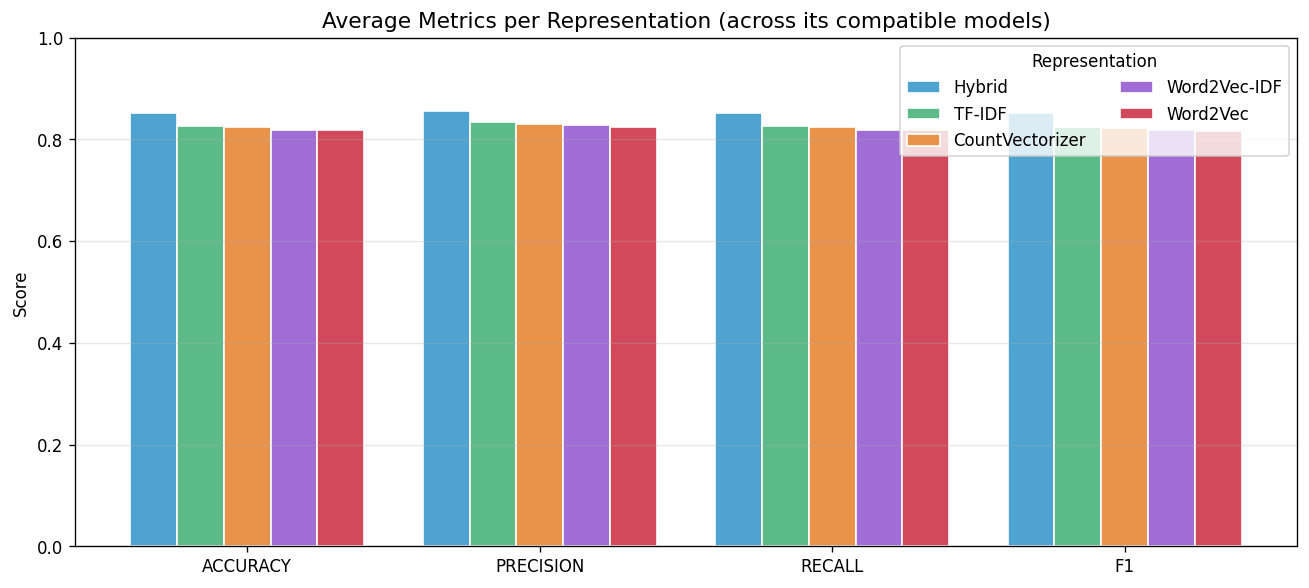
\includegraphics[width=0.75\textwidth]{../outputs/figures/avg_metrics_per_vectorizer.png}
    \caption{میانگین معیارها}
    \label{fig:vec_avg}
\end{figure}

\begin{figure}[H]
    \centering
    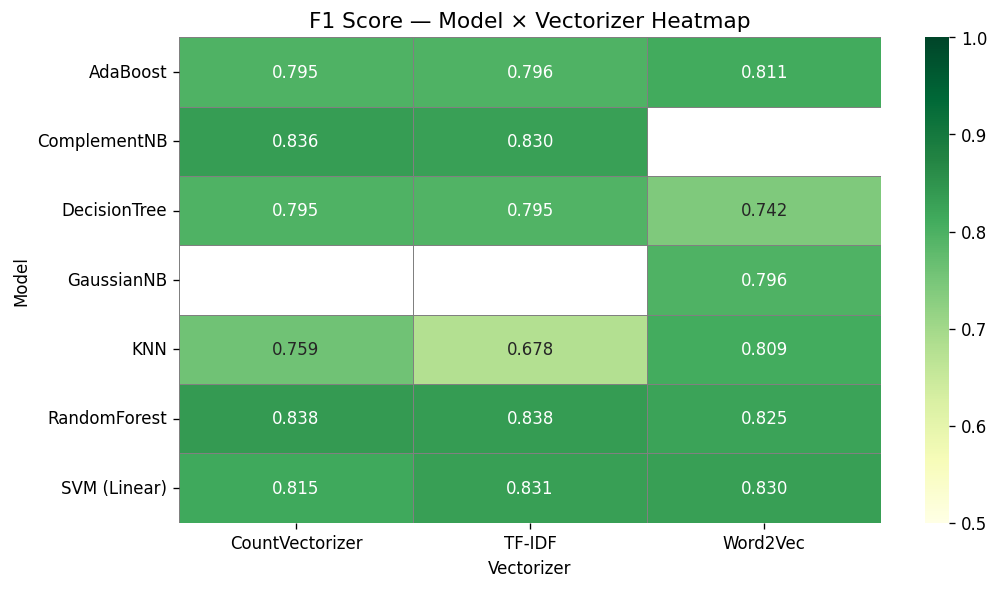
\includegraphics[width=0.75\textwidth]{../outputs/figures/f1_heatmap.png}
    \caption{هیت‌مپ \lr{F1}}
    \label{fig:f1_heatmap}
\end{figure}

\subsection{چرا \lr{Hybrid} انتخاب شد؟}

\lr{Hybrid} هم میانگین (\lr{0.8515}) هم اوج (\lr{0.8574}) رو برد. char n-gram املای غلط و پسوند فارسی رو می‌گیره؛ word TF-IDF هم عبارت‌هایی مثل \lr{NEG\_خوب} رو نگه می‌داره. بین سه روش \textbf{اجباری}، \lr{TF-IDF} برنده‌ست (\lr{0.8551} اوج)، نه \lr{CountVectorizer} (\lr{0.8501}). \lr{Hybrid} در عمل نسخه تقویت‌شده \lr{TF-IDF} با char union هست.

پس برای فاز \lr{Stacking}، \lr{Hybrid} ذخیره شد (\lr{best\_vectorizer.json}).


\section{فاز پنجم: \lr{Stacking}}

\subsection{طراحی}

چهار پایه روی \lr{Hybrid} sparse: \lr{ComplementNB}، \lr{SVM} کالیبره، \lr{LogisticRegression}، \lr{RandomForest} (\lr{n\_estimators=300}). \lr{meta-learner}: \lr{LogisticRegression}، \lr{cv=5}، \lr{stack\_method=auto}. زمان آموزش حدود \lr{683} ثانیه (\lr{11.4} دقیقه).

\subsection{نتایج}

\begin{table}[H]
\centering
\begin{tabular}{lcccc}
\toprule
\textbf{مدل} & \textbf{دقت} & \textbf{صحت} & \textbf{فراخوانی} & \textbf{\lr{F1}} \\
\midrule
\lr{Stacking} (\lr{Hybrid}) & \lr{0.8580} & \lr{0.8601} & \lr{0.8580} & \lr{0.8578} \\
\lr{SVM (tuned)} (تکی) & \lr{0.8578} & \lr{0.8620} & \lr{0.8578} & \lr{0.8574} \\
\bottomrule
\end{tabular}
\caption{\lr{Stacking} در برابر بهترین تکی}
\label{tab:stacking_results}
\end{table}

بهبود \lr{F1}: \lr{+0.0004} (\lr{0.04} نقطه درصد). کم ولی مثبت.

\begin{figure}[H]
    \centering
    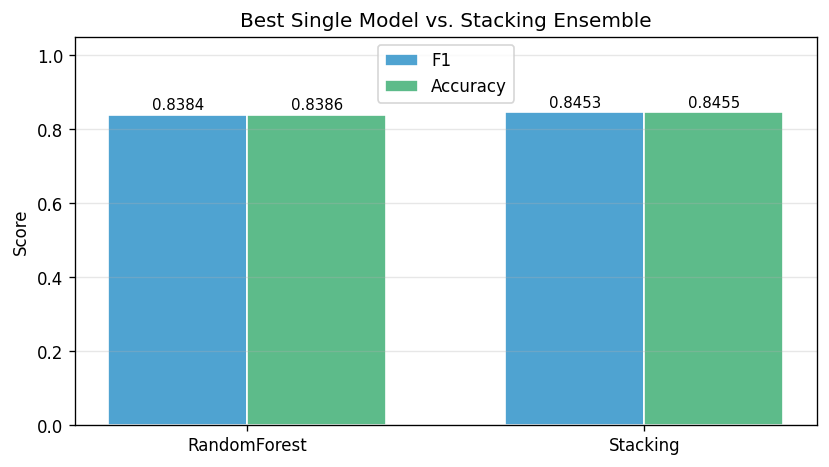
\includegraphics[width=0.65\textwidth]{../outputs/figures/stacking_vs_best.png}
    \caption{مقایسه \lr{Stacking} و بهترین تکی}
    \label{fig:stacking_vs_best}
\end{figure}

\begin{figure}[H]
    \centering
    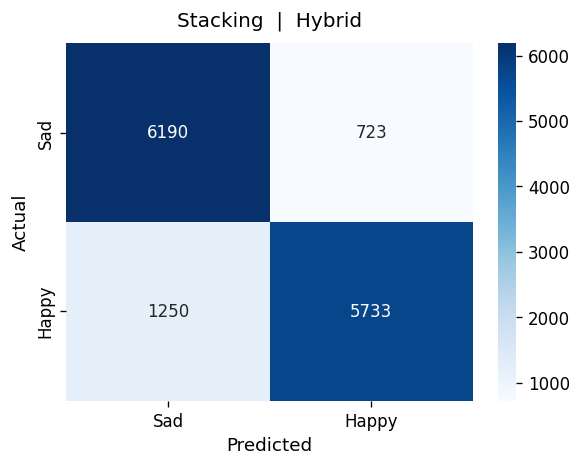
\includegraphics[width=0.55\textwidth]{../outputs/confusion_matrices/Stacking_Hybrid.png}
    \caption{ماتریس درهم‌ریختگی \lr{Stacking + Hybrid}}
    \label{fig:stacking_cm}
\end{figure}

\subsection{تحلیل}

\lr{Stacking} کمی بهتر از \lr{SVM tuned} شد. بهبود کوچیکه چون پایه‌ها روی یه ماتریس مشترک آموزش دیدن و \lr{SVM} خودش از قبل خیلی قوی بود. ولی \lr{meta-learner} یاد گرفته کی به کدوم پایه اعتماد کنه.

\subsection{نمونه‌های خطا و سقف دقت}

\begin{table}[H]
\centering
\small
\begin{tabularx}{\textwidth}{X c c}
\toprule
\textbf{متن} & \textbf{برچسب} & \textbf{پیش‌بینی} \\
\midrule
کیفیت خوب بود ولی نسبت به قیمت حجم غذا خوب بود & \lr{SAD} & \lr{HAPPY} \\
هسته زردآلو خیلی بد بود ولی برگه هلو خوب بود & \lr{SAD} & \lr{HAPPY} \\
آدرس اشتباه فرستاد ولی خود همبرگر خوب بود & \lr{SAD} & \lr{HAPPY} \\
از نظر مزه خوشمزه بود ولی حجم کم بود & \lr{SAD} & \lr{HAPPY} \\
سالاد سزار کاهو موند؛ سیب‌زمینی خوب بود & \lr{HAPPY} & \lr{SAD} \\
چیپس پنیر بدون سس تند سفارش دادم ولی تند فرستادید & \lr{HAPPY} & \lr{SAD} \\
\bottomrule
\end{tabularx}
\caption{خطاهای واقعی \lr{Stacking}}
\label{tab:stacking_examples}
\end{table}

حدود \lr{1,970} خطا از \lr{13,896} تست (\lr{85.8\%} دقت). خیلیاشون نظر مختلط یا برچسب مشکوک‌ان، نه خطای تصادفی مدل. «کیفیت عالی. اما غذا سرد شده بود» (\lr{HAPPY}) یا «خوشمزه بود ولی فوق العاده سرد» (\lr{SAD}) نمونه‌ان که انسان هم مردد میشه.

پس \lr{F1} حدود \lr{0.86} هم موفقیت pipeline کلاسیکه هم یادآوری که داده \lr{100\%} درست  نیست.


\section{فاز ششم (bonus): \lr{ParsBERT}}

بعد از اینکه \lr{Stacking Hybrid} به \lr{F1=0.8578} رسید، سقف مدل‌های کلاسیک روی \lr{bag-of-words} مشخص شد. فاز ۶ رفته سراغ \lr{transformer} فارسی تا ببینیم context و fine-tuning چقدر می‌تونه از این سقف بالاتر بره. همه نتایج این بخش از نوت‌بوک \lr{06\_parsbert.ipynb} روی \lr{Kaggle GPU} اومده.

\subsection{\lr{ParsBERT} چیه و چرا اصلاً امتحانش کردیم؟}

\lr{ParsBERT}\footnote{\lr{BERT} (\lr{Bidirectional Encoder Representations from Transformers}): مدل زبانی \lr{Transformer} دوطرفه. \lr{ParsBERT} نسخه فارسی‌ش هست که روی متن فارسی \lr{pretrain} شده.} یه \lr{language model} مبتنی بر \lr{Transformer} هست که روی حجم زیادی متن فارسی \lr{pretrain} شده. برخلاف \lr{CountVectorizer}/\lr{TF-IDF} که هر کلمه رو جدا می‌بینه، \lr{ParsBERT} جمله رو \textbf{دوطرفه} می‌خونه: معنی «خوب» وقتی قبلش «نه» یا «ولی» باشه با حالت ساده فرق می‌کنه. برای نظرات \lr{Snapfood} که پر از «خوب بود ولی...» هستن، همین تفاوت مهمه.

مدلی که استفاده کردیم \lr{HooshvareLab/bert-base-parsbert-uncased} هست — \lr{12} لایه \lr{Transformer}، hidden size \lr{768}، tokenizer خودش (\lr{WordPiece}). توی پیاده‌سازی ما (\lr{src/bert\_features.py}) embeddingها \textbf{روی متن خام} \lr{comment} ساخته میشن، نه روی خروجی پیش‌پردازش فاز ۱. دلیلش اینه که \lr{ParsBERT} با فارسی طبیعی \lr{pretrain} شده؛ مارکرهای \lr{NEG\_}/\lr{EMO\_} و پاکسازی سنگین فاز ۱ برای \lr{BERT} لزوماً کمک نمی‌کنه و گاهی گیجش می‌کنه.

\subsection{پیاده‌سازی و محیط اجرا}
نوت‌بوک روی \lr{Kaggle} اجرا شد. featureهای frozen از قبل کش شده بودن (\lr{X\_train\_bert.npy}، \lr{X\_test\_bert.npy} — هر کدوم \lr{768} بعد برای \lr{55,583} train و \lr{13,896} test). استخراج feature با \lr{ParsBertFeatureExtractor}: \lr{max\_length=128}، \lr{batch\_size=32}، \lr{pooling=mean} روی hidden stateهای واقعی (نه فقط \lr{[CLS]} خام)، چون برای frozen extraction معمولاً mean بهتر جواب میده.

سه مسیر جدا تست کردیم:
\textbf{مسیر ۱ — Frozen \lr{ParsBERT} + سرهای کلاسیک.} وزن‌های \lr{Transformer} ثابت موندن؛ فقط classifierهای \lr{sklearn} روی بردار \lr{768}-بعدی آموزش دیدن: \lr{SVM (Linear)} کالیبره، \lr{LogisticRegression}، \lr{HistGradientBoosting}. بعد همون سه تا رو با \lr{StackingClassifier} (\lr{meta-learner} = \lr{LogisticRegression}، \lr{cv=5}) ترکیب کردیم. آموزش stacking روی dense \lr{768}-بعدی حدود \lr{3633} ثانیه (\lr{60} دقیقه) طول کشید.

\begin{table}[H]
\centering
\small
\begin{tabular}{lcc}
\toprule
\textbf{مدل (frozen)} & \textbf{\lr{F1}} & \textbf{دقت} \\
\midrule
\lr{SVM (Linear)} & \lr{0.8445} & \lr{0.8447} \\
\lr{LogisticRegression} & \lr{0.8438} & \lr{0.8440} \\
\lr{HistGradientBoosting} & \lr{0.8357} & \lr{0.8361} \\
\lr{Stacking} & \lr{0.8450} & \lr{0.8452} \\
\bottomrule
\end{tabular}
\caption{نتایج frozen \lr{ParsBERT} + مدل‌های کلاسیک}
\label{tab:parsbert_frozen}
\end{table}

هیچکدوم از اینا از \lr{Stacking Hybrid} فاز ۵ (\lr{0.8578}) بالاتر نرفت. یعنی embedding از پیش آموزش‌دیده \textbf{به تنهایی} برای این دیتاست کافی نبود — حتی با stacking.

\textbf{مسیر ۲ — Fine-tune end-to-end.} اینجا کل \lr{ParsBERT} روی برچسب‌های \lr{Snappfood} fine-tune شد (\lr{BertForSequenceClassification}، \lr{num\_labels=2}). train به \lr{90\%} (\lr{50,024} نمونه) و \lr{10\%} (\lr{5,559} نمونه) برای validation داخل train شکستیم (\lr{random\_state=42}). hyperparameterها: \lr{3} epoch، \lr{batch\_size=32}، \lr{learning\_rate=2e-5}، \lr{weight\_decay=0.01}، \lr{fp16=True}، \lr{max\_length=128}. بهترین checkpoint با \lr{load\_best\_model\_at\_end} انتخاب شد.

نتیجه روی test: \lr{F1=0.8730}، دقت \lr{0.8731} — یعنی \lr{+0.0152} نسبت به \lr{Stacking Hybrid}. این اولین مدلی بود که مستقیم متن خام می‌خوند و از سقف کلاسیک عبور کرد.

\textbf{مسیر ۳ — Extended meta-ensemble.} پنج عضو قوی رو روی \lr{10\%} blend از train fit کردیم و probability خروجی‌شون رو به \lr{meta-learner} (\lr{LogisticRegression}، بهترین \lr{C=0.3}) دادیم: \lr{SVM} و \lr{LogReg} روی \lr{Hybrid}، \lr{HistGradientBoosting} روی frozen \lr{ParsBERT}، \lr{ComplementNB} روی word \lr{TF-IDF}، و fine-tuned \lr{ParsBERT}. \lr{meta-learner} روی blend \lr{10} بعدی probability (\lr{5} عضو در \lr{2} کلاس) آموزش دید. نتیجه test: \lr{F1=0.8713} — کمی پایین‌تر از fine-tune تنها (\lr{0.8730})، ولی هنوز خیلی بالاتر از pipeline کلاسیک. coefficientهای \lr{meta-learner} نشون میدن وزن اصلی روی fine-tuned \lr{ParsBERT} افتاده؛ اعضای کلاسیک بعد از اضافه شدن \lr{transformer} فاین‌تیون‌شده نقش کمتری دارن.

\subsection{مقایسه با baseline کلاسیک}

\begin{table}[H]
\centering
\begin{tabular}{lcc}
\toprule
\textbf{مرحله} & \textbf{\lr{F1}} & \textbf{نسبت به \lr{Stacking Hybrid}} \\
\midrule
\lr{Stacking Hybrid} (\lr{baseline}) & \lr{0.8578} & \lr{0} \\
\lr{ParsBERT frozen — stacking} & \lr{0.8450} & \lr{-0.0128} \\
\lr{ParsBERT fine-tuned} & \lr{0.8730} & \lr{+0.0152} \\
\lr{Extended ensemble} & \lr{0.8713} & \lr{+0.0135} \\
\bottomrule
\end{tabular}
\caption{خلاصه bonus در برابر \lr{baseline}}
\label{tab:parsbert}
\end{table}

\begin{figure}[H]
    \centering
    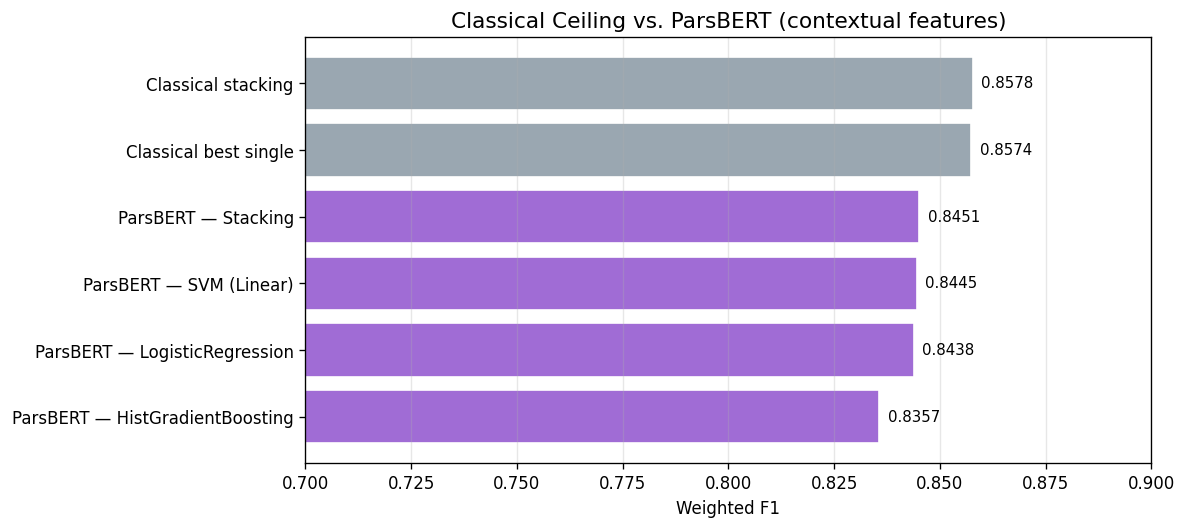
\includegraphics[width=0.85\textwidth]{../outputs/figures/parsbert_vs_classical.png}
    \caption{مقایسه \lr{ParsBERT} و pipeline کلاسیک}
    \label{fig:parsbert}
\end{figure}

\subsection{جمع‌بندی فاز ۶}

خوبیش چیه؟ fine-tune واقعاً سقف رو شکوند (\lr{+1.5} نقطه \lr{F1}). بدیش چیه؟ نیاز به \lr{GPU}، زمان آموزش بیشتر، و وابستگی به \lr{HuggingFace}/\lr{transformers}. frozen \lr{ParsBERT} حتی با stacking از \lr{Hybrid} ضعیف‌تر بود — پس «داشتن \lr{BERT}» به تنهایی کافی نیست؛ باید روی همین دامنه و همین برچسب‌ها fine-tune بشه.

پس در نهایت: برای عبور از سقف \lr{bag-of-words}، context لازمه؛ frozen کافی نیست، fine-tune لازمه. فاز ۶ bonus بود و deliverable اصلی پروژه همچنان فازهای ۱–۵ با مدل‌های کلاسیکه.


\section{نتیجه‌گیری}

یه pipeline کامل روی \lr{69,479} نظر \lr{Snapfood}: پیش‌پردازش احساس‌محور (نفی، \lr{emoji})، پنج \lr{vectorizer}، \lr{32+} آزمایش مدل، انتخاب \lr{Hybrid}، \lr{Stacking} با \lr{F1=0.8578}.

نکات کلیدی: \lr{URL} قبل از \lr{Hazm}؛ \lr{stopword} احساسی حذف نشه؛ \lr{Hybrid} برنده sparse؛ \lr{SVM tuned} قوی‌تر از درخت‌ها؛ \lr{Stacking} بهبود کوچک ولی مثبت؛ خطاها اغلب نظر مختلط/برچسب نویزی؛ \lr{ParsBERT} فاین‌تیون‌شده به \lr{0.8730} رسید.

تحویل اجباری پروژه با فازهای ۱–۵ کامله؛ فاز ۶ bonus و بهبود واقعی با \lr{transformer} فاین‌تیون‌شده بود.

\end{document}
